\chapter{Additional PMU Placement Proofs}
\label{ch:appendix-pmu}


In Chapter \ref{ch:pmu} we proved that \full (Section \ref{subsec:full}), \maxinc (Section \ref{subsec:maxinc}), \xval (Section \ref{subsec:xval}),
and \xvalpart (Section \ref{subsec:xvalpart}) are each NP-Complete when considering networks with both zero-injection and injection buses.  Here we prove that each problem is also NP-Complete
for graphs containing only zero-injection nodes.  The proofs closely resemble those in Sections \ref{subsec:full} - \ref{subsec:xvalpart}. % but do differ in their details. 
Then, we provide pseudo-code and complexity proofs for the approximation algorithms described in Section \ref{sec:approx}.  These proofs consider graphs with both zero-injection and injection buses. 


%We prove that the PMU Placement problems described in Chaper \ref{ch:pmu}: \full (Section \ref{subsec:full}), \maxinc (Section \ref{subsec:maxinc}), \xval (Section \ref{subsec:xval}),
%and \xvalpart (Section \ref{subsec:xvalpart}) are NP-Complete when considering 

\section{NP-Completeness Proofs for PMU Placement in Zero-Injection Graphs}

In the following order \maxinc (Section \ref{subsec:zero-maxinc}), \xval (Section \ref{subsec:zero-xval}), and \xvalpart (Section \ref{subsec:zero-xvalpart}), 
we prove that each problem is NP-Complete for graphs containing only zero-injection nodes.  Our proofs below do not explicitly mention our assumption that all nodes 
are zero-injection; rather, %our liberal use of observability rule 2 implies our implicit assumption that all nodes are zero-injection.
this assumption is implicit in the fact that we apply observability rule 2 whenever possible.
We omit a new proof for \full because Brueni and Heath \cite{Brueni05} prove \full is NP-Complete for zero-injection graphs.  

Our proofs follow the same strategy outlined in Section \ref{subsec:proofstrat}: we reduce for \sat to show each problem is NP-Complete.  
Recall that our proofs from Chapter \ref{ch:pmu} relied on the definition of a bipartite 
graph $G(\phi)=(V(\phi),E(\phi))$ where $\phi$ is a 3-SAT formula with variables $\{v_1,v_2, \dots , v_r\}$ and clauses $\{c_1,c_2, \dots , c_s \}$.  
$G(\phi)$'s vertices and edges were defined as follows:
\begin{eqnarray*}
% \nonumber to remove numbering (before each equation)
 V(\phi) &= &\{v_i\; \vert\; 1 \leq i \leq r \} \cup \{c_j \;\vert\; 1 \leq j \leq s \} \\
 E(\phi) &=& \{ (v_i,c_j)\;\vert\; v_i \in c_j\;\; or \;\; \overline{v_i} \in c_j\}.
\end{eqnarray*}


\subsection{\maxinc Problem for Zero-Injection Graphs}
\label{subsec:zero-maxinc}

\begin{figure}[t]
  \begin{center}
    \fbox{\subfigure[Variable gadget $V_i$.The dashed edges are connections to clause gadgets.]{\label{fig:zero-variable-gadget}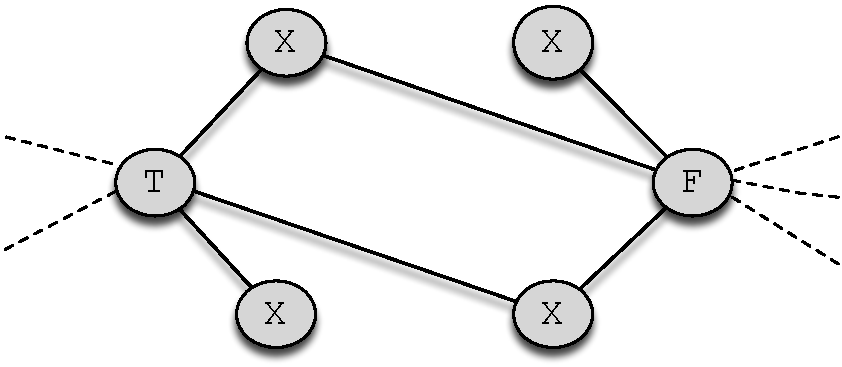
\includegraphics[scale=0.30]{figs/variable-gadget.pdf}}}
    \fbox{\subfigure[Clause gadget $C_j$. The dashed edges are connections to variable gadgets.]{\label{fig:zero-clause-gadget}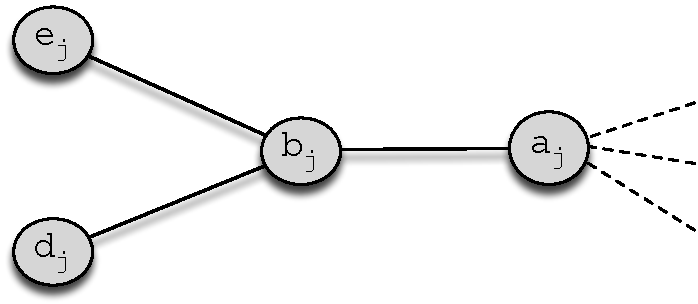
\includegraphics[scale=0.30]{figs/proof1b.pdf}}}
  \end{center}
	\caption{Gadgets used in Theorem \ref{thm:zero-npc-maxinc} proof.}
  \label{fig:zero-maxinc}
\end{figure}

A description of \maxinc can be found in Section \ref{subsec:maxinc}.  Our proof for the theorem below (Theorem \ref{thm:zero-npc-maxinc}) is similar to that for Theorem \ref{thm:npc-maxinc}.
\begin{theorem}
\maxinc is NP-Complete when considering graphs with only zero-injection nodes.  %even when restricted to the class of bipartite planar graphs.
\label{thm:zero-npc-maxinc}
\end{theorem}

{\bf Proof idea:} First, we construct problem-specific gadgets for variables and clauses. We then demonstrate that any solution that observes $m$ nodes must place the PMUs only on nodes in the variable gadgets. Next we show that as a result of this, the problem of observing $m$ nodes in this graph reduces to the NP-complete problem presented in \cite{Brueni05}, which concludes our proof.

\begin{proof}
We start by arguing that \maxinc $\in \mathcal{NP}$. First, nondeterministically select $k$ nodes in which to place PMUs. Then we use the rules specified in Section \ref{subsec:observe} to determine
the number of observed nodes. 

We reduce from \sats, where $\phi$ is an arbitrary \sat formula, to show \maxinc is NP-hard.
Specifically, given a graph $G(\phi)$ we construct a new graph $H_1(\phi) = (V_1(\phi), E_1(\phi))$ by replacing each variable 
(clause) node in $G(\phi)$ with the variable (clause) gadget shown in Figure \ref{fig:zero-variable-gadget} (\ref{fig:zero-clause-gadget}). The edges connecting clause gadgets 
with variable gadgets express which variables are in each clause: for each clause gadget $C_j$, node $a_j$ is attached to node $T$ in variable gadget $V_i$ if, in $\phi$, $v_i$ is in $c_j$,
and to node $F$ if $\overline{v_i}$ is in $c_j$. For convenience, we let $G=H_1(\phi)$.

With this construct in place, we move on to our proof. Here we consider the case of  $k=r$ and $m = 6r + 2s$, and show that $\phi$ is satisfiable if and only if $r=|\Phi_G|$ PMUs 
can be placed on $G$ such that $m \leq |\Phi^R_{G}| < |V|$. We will later discuss how to extend this proof for any larger value of $m$.  %cover $m$ nodes in $G'$.

$(\Rightarrow)$ Assume $\phi$ is satisfiable by truth assignment $A_{\phi}$. Then, consider the placement $\Phi_G$ s.t. for each variable gadget $V_i$, $T_i\in \Phi_G \Leftrightarrow v_i=True$ 
in $A_\phi$, and  $F_i\in \Phi_G \Leftrightarrow v_i=False$. It has been shown in \cite{Brueni05} that for $H(\phi)$ this placement observes all $H(\phi)$, and it can be easily verified that
all nodes in $H_1(\phi)$ are observed as well except for $d_j, e_j$ for each $C_j$. This amounts to $2s$ nodes, so exactly $m$ nodes are observed by $\Phi_G$, as required.  

$(\Leftarrow)$ 
We begin by proving that any solution that observes $m$ nodes must place the PMUs only on nodes in the variable gadgets. Assume that there are $1<t\leq r$ variable gadgets without a PMU. 
Then, at most $t$ PMUs are on nodes in clause gadgets, so {\it at least} $\max(s-t,0)$ clause gadgets are without PMUs. We want to show here that for $m=6r+2s$, $t=0$.

To prove this, we rely on the following two simple observations:
\begin{itemize}
	\item In any variable gadget $V_i$, nodes $X$ (Figure \ref{fig:zero-variable-gadget}) cannot be observed unless  there is a PMU somewhere in $V_i$. Note that there are $4$ such nodes per $V_i$.
	\item In any clause gadget $C_j$, nodes $e_j$ and $d_j$ cannot be observed unless there is a PMU somewhere in $C_j$. Note that there are $2$ such nodes per $C_j$. 
\end{itemize}
Thus, given some $t$, the number of unobserved nodes is {\it at least} $4t + \max(2(s-t), 0)$. However, since $|V|-m \leq 2s$, there are {\em at most}  $2s$ unobserved nodes. So we get 
$2s \geq 4t + \max(2(s-t), 0)$. We consider two cases:
\begin{itemize}
	\item $s\geq t$: then we get $2s \geq 2s+2t \Rightarrow t=0.$
	\item $s < t$:	then we get $2s \geq 4t \Rightarrow s\geq 2t$, and since we assume here $0\leq s < t$ this leads to a contradiction and so this case cannot occur.
\end{itemize}

Thus, we have concluded that the $r$ PMUs must be on nodes in variable gadgets, all of which, it is important to note, were also part of the original $H(\phi)$ graph. 
We return to this point shortly. 

We now observe that for each clause gadget $C_j$, such a placement of PMUs cannot observe nodes of type  $e_j, d_j$, which amounts to a total of $2s$ unobserved nodes - the allowable bound.
This means that all other nodes in $G$ must be observed. Specifically, this is exactly all the nodes in the original $H(\phi)$ graph, and PMUs can only be placed on variable gadgets, 
all of which are included in $H(\phi)$ as well. Thus, the problem reduces to the problem in \cite{Brueni05}. 
We use the proof in \cite{Brueni05} to determine that all clauses in $\phi$ are satisfied by the truth assignment derived from $\Phi_G$. 
\end{proof}



\begin{figure}[t]
\centering
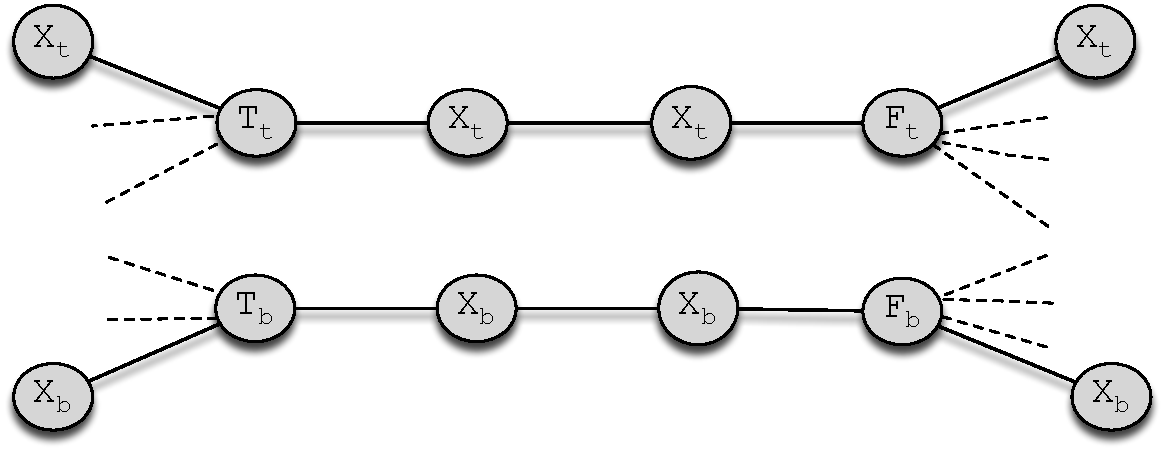
\includegraphics[scale=0.46]{figs/xvalgadget2.pdf}
\caption{Variable gadget used in Theorem \ref{thm:zero-npc-xval} proof. The dashed edges are connections to clause gadgets.} 
\label{fig:zero-xval-gadget}
\end{figure}

\subsection{\xval Problem for Zero-Injection Graphs}
\label{subsec:zero-xval}

The problem statement for \xval can be found in Section \ref{subsec:xval}.  The proof for Theorem \ref{thm:zero-npc-xval}, below, closely follows the structure of Theorem \ref{thm:npc-xval}'s proof.

\begin{theorem}
\xval is NP-Complete when considering graphs with only zero-injection nodes.   % even when restricted to the class of bipartite and chordal graphs.
\label{thm:zero-npc-xval}
\end{theorem}


\begin{proof}
First, we argue that \xval $\in \mathcal{NP}$.  Given a \xval solution, we use
the polynomial time algorithm described in our proof for Theorem
\ref{thm:zero-npc-maxinc} to determine if all nodes are observed.  Then, for each
PMU node we run a breadth-first search, stopping at depth $2$, to check that
the cross-validation rules are satisfied.

To show \xval is NP-hard, we reduce from \sats.  Our reduction is similar to
the one used in Theorem \ref{thm:zero-npc-maxinc}.  
For this problem, we use different variable and clause gadgets. The clause gadgets consist of the edge $(a_j, b_j)$ from Figure \ref{fig:zero-clause-gadget},
which are the same as used in \cite{Brueni05}. The new variable gadget is shown in Figure
\ref{fig:zero-xval-gadget}. As can be seen in this figure, the variable gadgets are comprised of two disconnected
subgraphs: we refer to the upper subgraph as $V_{it}$ and the
lower subgraph as $V_{ib}$. Clause gadgets are connected to a variable gadgets in the following manner: 
for each clause $c_j$ that contains variable $v_i$ in $\phi$, the corresponding clause gadget has the edges $(a_j, T_t), (a_j,
T_b)$, and for each clause $c_j$ that contains variable $\overline{v_i}$ in
$\phi$, the corresponding clause gadget has the edges $(a_j, F_t), (a_j,
F_b)$. We denote the resulting graph as $H_2(\phi)$, and for what follows assume $G=H_2(\phi)$.

We now show that $\phi$ is satisfiable if and only if
$k=2r$ PMUs can be placed on $G$ such that $G$ is fully observed under the
condition that all PMUs are cross-validated, and that $2r$ PMUs are the minimal 
bound for observing the graph with cross-validation.

$(\Rightarrow)$ Assume $\phi$ is satisfiable by truth assignment $A_{\phi}$.
For each $1\leq i\leq r$, if $v_i=True$ in $A_{\phi}$ we place a PMU at $T_b$
and at $T_t$ of the variable gadget $V_i$. Otherwise, we place a PMU at $F_b$
and at $F_t$ of this gadget. In either case, the PMU nodes in $V_i$ must be
adjacent to a clause node, making $T_t$ ($F_t$) two hops away from
$T_b$ ($F_b$). Therefore, all PMUs are cross-validated by XV2. 

Now we argue that $\Phi_G$ observes all $v \in V$:  
\begin{itemize}
  \item Consider a clause node $a_j$. Since $\phi$ is satisfied, for some
  index $i$ we have  $v_i \in c_j \wedge v_i\in A_{\phi}$ or $\overline{v_i} \in
  c_j \wedge \overline{v_i}\in A_{\phi}$. For the first case, the PMUs in $V_i$ are placed
  on $\{T_b, T_t\}$ and as a result $a_j$ is observed by applying O1 at $T_b$ or at  $T_t$. A similar argument applies for the second case. So, all $a_j$
  nodes are observed.

  \item Next, consider the nodes on the variable gadgets.  When $v_i \in A_{\phi}$,
  $T_t$'s neighbors, in $V_{it}$, are observed via O1.
  (the second case, $\overline{v_i} \in A_{\phi}$, follows by symmetry). 
  The remaining $V_{it}$ nodes are observed via O2 - note that if $F_t$ is connected to a clause gadget we know from the previous step this clause is observed. By symmetry of $V_{ib}$ and
  $V_{it}$, the same argument can be made for $V_{ib}$ to show all $V_{ib}$ nodes
  are observed.

 \item Finally, all the neighbors of $a_j$ in variable gadgets are observed, and $a_j$ is observed, so we can now apply O2 at each node $a_j$ to observe the remaining $b_j$ nodes.
\end{itemize}
This completes this direction of the theorem.

$(\Leftarrow)$ Suppose $\Phi_G$ observes all nodes in $G$
under the condition that each PMU is cross-validated, and that $|\Phi_G|=2r$. We want to show that
$\phi$ is satisfiable by the truth assignment derived from $\Phi_G$. We prove this by showing
that (a) each variable gadget must have exactly $2$ PMUs and (b) there must be
a PMU at each subgraph of the variable gadget. Once (b) is shown, (c)
cross-validation restrictions force the PMUs to be either on both
$T$-nodes or both $F$-nodes. We conclude by showing that (d) the PMU nodes correspond
to true/false assignments to variables which satisfy $\phi$.

We begin by showing that each variable gadget must have $2$ PMUs. Let
$V_i$ be a variable gadget with less than two PMUs. By placing PMUs on
clause gadgets attached to $V_i$, at most we can observe $T_t, T_b, F_t$ and
$F_b$ directly from the clause gadgets. Next, at least one of the $V_i$
subgraphs has no PMU: without loss of generality, let this be $V_{it}$. 
We cannot apply O1 at $T_t$ or $F_t$,
since they have no PMU. We cannot apply O2 at these nodes since they each have
two unobserved $X_t$ nodes. Thus, all $X_t$ nodes are unobserved in $V_{it}$,
contrary to our assumption that the entire graph is observed. Thus we have
shown that there must be at least $2$ PMUs at each variable gadget. Also 
it is clear from this proof that, in fact, there must be at least one PMU in each subgraph of each
variable gadget. Finally, since there are $2r$ PMUs and $r$ variables, we conclude that 
each variable gadget has exactly two PMUs -- one PMU for each variable gadget subgraph --
and there are no PMUs on clause nodes.
%accounts for all the PMUs - no PMUs on clause nodes.

Due to the cross-validation constraint, it is clear that a PMU on $V_{it}$ can only
be cross-validated by a PMU on $V_{ib}$ (since all other variable-gadgets are
more than $2$ hops away), and specifically this would require both to be either
on $\{T_t, T_b\}$ or $\{F_t, F_b\}$. 

Without loss of generality, assume for an arbitrary variable gadget, $V_i$, 
we placed the PMUs at $\{T_t, T_b\}$. By applying O1 and O2, this
placement can observe all nodes in the variable gadget if $\{F_t, F_b\}$ in this gadget
are not adjacent to a clause node. If they are adjacent to some $a_h$ node, each of $\{F_t, F_b\}$ can observe its adjacent leaf-$X$-node only via O2, and only if
$a_h$ is already observed. Since we are given a PMU placement that observes the entire
graph, this implies that $a_h$ is indeed observed and thus adjacent to some variable node with a PMU,
such that O1 could be applied to view $a_h$. Assume without loss of generality,
$a_h$ is adjacent to PMU nodes $T_b,T_t$ from variable gadget $V_l$, then the clause $c_h \in \phi$ is
satisfied if $v_l$ is true. A similar argument can be made if $V_l$ is adjacent to
PMU nodes $F_t, F_b$. We conclude that all clauses in $\phi$ are satisfied by
the truth assignment derived from $\Phi_G$.
\end{proof}



\subsection{\xvalpart Problem for Zero-Injection Graphs}
\label{subsec:zero-xvalpart}

The \xvalpart problem is described in Section \ref{subsec:xvalpart}.  The proof below for Theorem \ref{thm:zero-npc-xvalpart} closely resembles the proof for Theorem \ref{thm:npc-xvalpart}.

\begin{theorem}
\xvalpart is NP-Complete when considering graphs with only zero-injection nodes.   % even when restricted to the class of bipartite and chordal graphs.
\label{thm:zero-npc-xvalpart}
\end{theorem}


{\bf Proof Idea:} We show \xvalpart is NP-hard by reducing from \sats. Our proof is a combination of the NP-hardness proofs for \maxinc and \xvals. 
From a \sat formula, $\phi$, we create a graph $G=(V,E)$ with the clause gadgets from \maxinc (Figure \ref{fig:zero-clause-gadget}) and the variable gadgets from \xval (Figure \ref{fig:zero-xval-gadget}).
The edges in $G$ are identical the ones the graph created in our reduction for \xvals. 

We show that any solution that observes $m=|V|-2s$ nodes must place the PMUs exclusively on nodes in the variable gadgets. As a result, we show
$2$ nodes in each clause gadget -- $e_j$ and $d_j$ for clause $C_j$ -- are not observed, yielding a total $2s$ unobserved nodes. This implies all other nodes must be 
observed, and thus reduces our problem to the scenario considered in Theorem \ref{thm:zero-npc-xval}, which is already proven.


\begin{proof}
\xvalpart is easily in $\mathcal{NP}$. We verify a \xvalpart solution using the same polynomial time algorithm described in our proof 
for Theorem \ref{thm:zero-npc-xval}. % used to verify an \xval solution.

We reduce from \sat to show \xvalpart is NP-hard. Our reduction is a combination
of the reductions used for \maxinc and \xvals. Given a \sat formula, $\phi$,
with variables $\{v_1,v_2, \dots , v_r\}$ and the set of clauses $\{c_1,c_2,
\dots , c_s \}$, we form a new graph, $H_3(\phi) = (V(\phi),E(\phi))$  as follows. Each clause $c_j$
corresponds to the clause gadget from \maxinc (Figure \ref{fig:zero-clause-gadget}) 
and the variable gadgets from \xval (Figure \ref{fig:xval-gadget}). 
As in Theorem \ref{thm:zero-npc-xval}, we refer to the upper subgraph of variable gadget, $V_i$, 
as $V_{it}$ and the lower subgraph as $V_{ib}$.  Also, we let $H_3(\phi) = G=(V,E)$.

Let $k = 2r$ and $m = 12r + 2s = |V| - 2s$. As in our NP-hardness proof for \maxincs, $m$ includes all nodes in $G$
except $d_j,e_j$ of each clause gadget. We need to show that $\phi$ is satisfiable if and only if
$2r$ cross-validated PMUs can be placed on $G$ such that $m \leq |\Phi^R_{G}| < |V|$.

$(\Rightarrow)$ Assume $\phi$ is satisfiable by truth assignment $A_{\phi}$.
For each $1\leq i\leq r$, if $v_i=True$ in $A_{\phi}$ we place a PMU at $T_b$
and at $T_t$ of the variable gadget $V_i$. Otherwise, we place a PMU at $F_b$
and at $F_t$ of this gadget. In either case, the PMU nodes in $V_i$ must be
adjacent to a clause node, making $T_t$ ($F_t$) two hops away from
$T_b$ ($F_b$). Therefore, all PMUs are cross-validated by XV2. 

This placement of $2r$ PMUs, $\Phi_G$, is exactly the same one derived from $\phi$'s satisfying instance in Theorem \ref{thm:zero-npc-xval}.
Since $\Phi_G$ only has PMUs on variable gadgets, all $a_j$ and $b_j$ nodes are observed by the same argument used in Theorem \ref{thm:zero-npc-xval}.
Thus, at least $12r + 2s$ nodes are observed in $G$.
Because no PMU in $\Phi_G$ is placed on a clause gadget, $C_j$, we know that all $e_j$ and $d_j$ are not observed. 
We conclude that exactly $m$ nodes are observed using $\Phi_G$.

$(\Leftarrow)$ 
We begin by proving that any solution that observes $m$ nodes must place the PMUs only on nodes in the variable gadgets. Assume that there are $1<t\leq r$ variable gadgets without a PMU. 
Then, at most $t$ PMUs are on nodes in clause gadgets, so {\it at least} $\max(s-t,0)$ clause gadgets are without PMUs. We want to show here that for $m=12r+2s$, $t=0$.

To prove this, we rely on the following observations:
\begin{itemize}
	\item As shown in Theorem \ref{thm:zero-npc-xval}, a variable gadget's subgraph with no PMU has at least $4$ unobserved nodes.
	\item In any clause gadget $C_j$, nodes $e_j$ and $d_j$ cannot be observed if there is no PMU somewhere in $C_j$. Note that there are $2$ such nodes. 
\end{itemize}
Thus, given some $t$, the number of unobserved nodes is {\it at least} $4t + \max(2(s-t), 0)$. However, since $|V|-m \leq 2s$, there are {\em at most}  $2s$ unobserved nodes. So we get 
$2s \geq 4t + \max(2(s-t), 0)$. We consider two cases:
\begin{itemize}
	\item $s\geq t$: then we get $2s \geq 2s+2t \Rightarrow t=0.$
	\item $s < t$:	then we get $2s \geq 4t \Rightarrow s\geq 2t$, and since we assume here $0\leq s < t$ this leads to a contradiction and so this case cannot occur.
\end{itemize}

Thus, we have concluded that the $2r$ PMUs must be on variable gadget. %, which, it is important to note, were also part of the original $H(\phi)$ graph. We shall return to this point shortly. 
We now observe that for each clause gadget $C_j$, such a placement of PMUs cannot observe nodes of type  $e_j, d_j$, which amounts to a total of $2s$ unobserved nodes - the allowable bound.
This means that all other nodes in $G$ must be observed. Specifically this is exactly all the nodes in $H_2(\phi)$ from the Theorem \ref{thm:zero-npc-xval} proof, and PMUs can only be placed on 
variable gadgets, all of which are included $H_2(\phi)$ from the Theorem \ref{thm:zero-npc-xval} proof. Thus, the problem reduces to the problem in Theorem \ref{thm:zero-npc-xval} and so we 
the Theorem \ref{thm:zero-npc-xval} proof to determine that all clauses in $\phi$ are satisfied by the truth assignment derived from $\Phi_G$. 
\end{proof}



\subsection{Extending Gadgets to Cover a Range of $m$ and $|V|$ values}
\label{subsec:zero-extend}

In the \xvalpart and \maxinc proofs we demonstrated NP-completeness for $m=|V|-2s$. 
We show that slight adjustments to the variable and clause gadgets can yield a much wider range of $m$ and $|V|$ values. 
We present the outline for new gadget constructions and leave the detailed analysis to the reader.

To increase the size of $m$ (e.g., the number of observed nodes), we simply add more $X$ nodes between the $T$ and $F$ nodes in the variable gadgets used in our proofs for \xvalpart and \maxincs. 
The new variable gadgets for \maxinc and \xvalpart are shown in Figure \ref{fig:zero-variable-extend1} and Figure \ref{fig:zero-variable-extend2}, respectively.
The same PMU placement described in the NP-Completeness proofs for each problem observes these newly introduced nodes.

In order to increase the size of $|V|$ while keeping $m$ the same, we replace each clause gadget, $C_j$ for $1 \leq j \leq s$, with a new clause gadget, $C_j'$,
shown in Figure \ref{fig:zero-clause-extend}. 
For \maxincs, the optimal placement of PMUs on $C_j'$ is to place PMUs on every fourth $b_{j,h}$ node, as shown in Figure \ref{fig:zero-clause-extend-observe}. 
As a result, the optimal placement of $l$ PMUs on $C_j'$ can at most observe $6l$ nodes.  By adding $6l$ $T$ nodes to each variable gadget, more nodes 
are always observed by placing a PMU on the variable gadget rather than at a clause gadget. We can use this to argue that PMUs are only placed on variable gadgets and then leverage the 
argument from Theorem \ref{thm:zero-npc-maxinc} to show \maxinc is NP-Complete for any $\frac{m}{|V|}$. A similar argument can be made for \xvalparts.

\begin{figure}[t]
  \begin{center}
    \subfigure[Extended variable gadget used for \maxincs.]{\label{fig:zero-variable-extend1}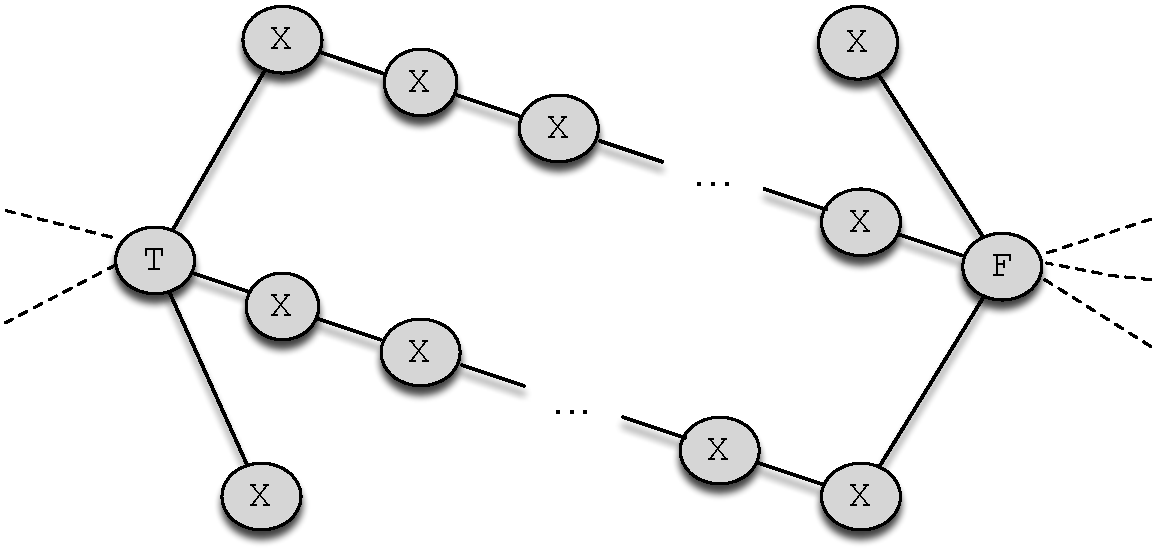
\includegraphics[scale=0.41]{figs/variable-gadget-extend.pdf}}
    \subfigure[Extended variable gadget used for \xvalparts.]{\label{fig:zero-variable-extend2}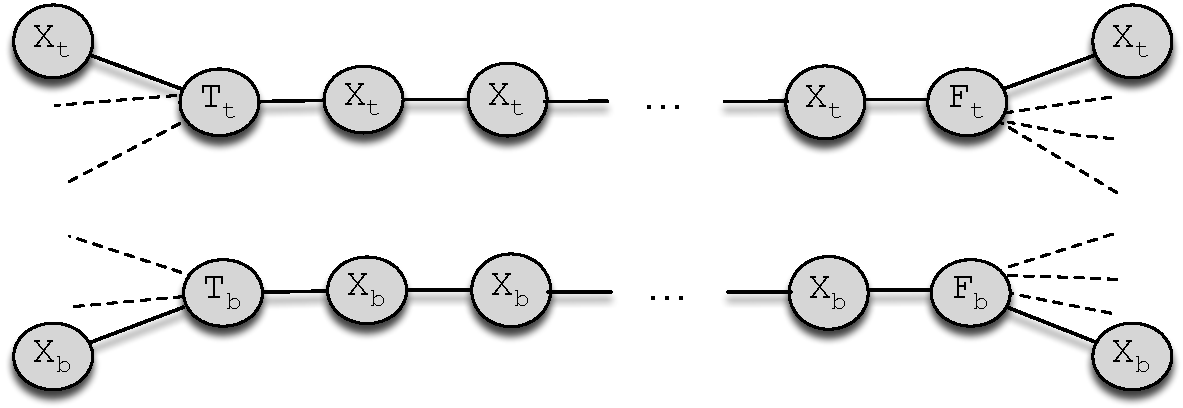
\includegraphics[scale=0.41]{figs/xvalgadget2-extend.pdf}}
  \end{center}
	\caption{Figures for variable gadget extensions described in Section \ref{subsec:zero-extend}. The dashed edges indicate connections to clause gadget nodes. }
  \label{fig:zero-clause-extended}
\end{figure}


\begin{figure}[t]
  \begin{center}
    \subfigure[Extended clause gadget $C_j$.]{\label{fig:zero-clause-extend}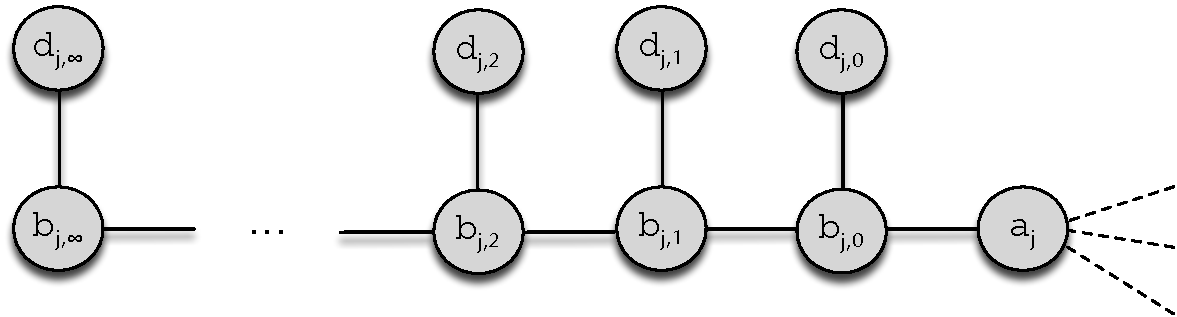
\includegraphics[scale=0.41]{figs/clausegadget-extension.pdf}}
    \subfigure[Observed nodes in extended clause gadget $C_j$ shown in (a).  PMU nodes are dark gray, nodes observed by O2 have a dashed border, and all other
	nodes are observed by O1.]
	{\label{fig:zero-clause-extend-observe}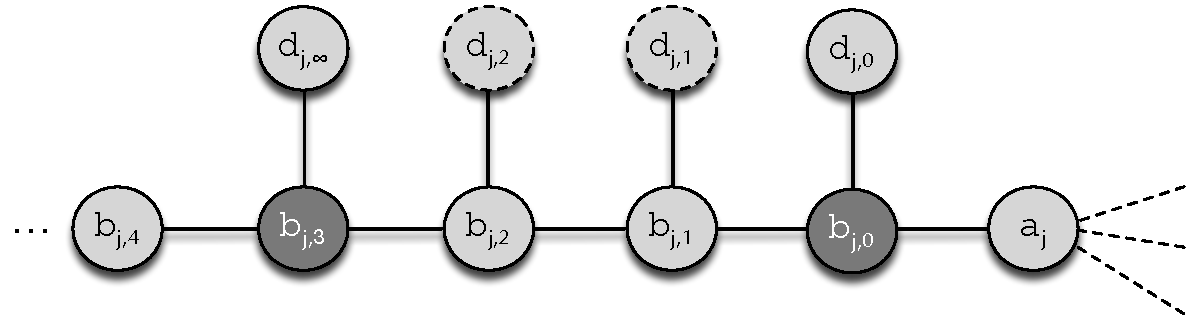
\includegraphics[scale=0.41]{figs/clausegadget-extension-observe.pdf}}
  \end{center}
	\caption{Figures for clause gadget extensions described in Section \ref{subsec:zero-extend}. The dashed edges indicate connections to variable gadget nodes. }
  \label{fig:zero-clause-extended}
\end{figure}

\section{Approximation Algorithm Complexity Proofs}
\label{sec:appendix-approx}

In Section \ref{sec:approx} we presented two greedy approximation algorithms, {\tt greedy} and {\tt xvgreedy}, that iteratively add a PMU in each step to the node that
observes the maximum number of new nodes.  Here the pseudo-code for each algorithm is specified and we prove that each algorithm has polynomial time complexity.  We emphasize
that these algorithms, unlike the problems discussed in the previous section, make no assumptions that nodes must be zero-injection.

The pseudo-code for {\tt greedy} and {\tt xvgreedy} can be found in Algorithm \ref{alg:greedy} and Algorithm \ref{alg:xvgreedy}, respectively.

\begin{algorithm}
\caption{{\tt greedy} with input $G=(V,E)$ and $k$ PMUs}
\label{alg:greedy}

\begin{algorithmic}[1]

\STATE{$\Phi_G \leftarrow \emptyset$}
\FOR{$k$ iterations}
	\STATE{$maxObserved \leftarrow 0$}
	\FOR{{\bf each} $v \in (V - \Phi_G$)}
		\STATE{$numObserved \leftarrow 0$}
		\FOR{{\bf each} $u \in (\Phi_G \cup \{v\})$}
			\STATE{add PMU to $u$}
			\STATE{apply O1 at $u$ and update $numObserved$}
		\ENDFOR
		\REPEAT
			\STATE{$flag \leftarrow False$}
			\FOR{{\bf each} $w \in (V - (\Phi_G \cup \{v\}))$}
				\IF{$w \in (V_Z \cap \Phi_G^R)$ and $w$ has $1$ unobserved neighbor}
					\STATE{apply O2 at $w$ and update $numObserved$}
					\STATE{$flag \leftarrow True$}
				\ENDIF
			\ENDFOR
		\UNTIL{$flag = False$}
		\IF{$numObserved > maxObserved$}
			\STATE{$greedyNode \leftarrow v$}
			\STATE{$maxObserved \leftarrow numObserved$}
		\ENDIF
	\ENDFOR
	\STATE{$\Phi_G \leftarrow \Phi_G \cup \{greedyNode\}$}
\ENDFOR
\end{algorithmic}
\end{algorithm}

\begin{theorem}
For input graph $G=(V,E)$ and $k$ PMUs {\tt greedy} has $O(dkn^3)$ complexity, where $n=|V|$ and $d$ is the maximum degree node in $V$.
\label{thm:app-greedy-complex}
\end{theorem}
\begin{proof}
%In our proof we implicitly refer to Algorithm \ref{alg:greedy} when referring to the steps of the algorithm.
%Specifically, when we refer to the {\tt greedy} algorithm steps we are referencing the Algorithm \ref{alg:greedy} steps.
The procedure to determine the number of nodes observed by a candidate PMU placement spans steps $6 - 18$.
{\footnote {\small In this proof, step $i$ refers to the $i^{th}$ line  in Algorithm \ref{alg:greedy}.}}
First, we apply O1 at each PMU node (steps $6 -9$). O1 takes $O(d)$ time 
to be applied at a single node.  Because $|\Phi_G| \leq k$, the total time to apply O1 is $O(dk)$. 

Then, we iteratively apply O2 (steps $10-18$), terminating when no new nodes are observed.  Like O1, applying O2 at a single node takes $O(d)$ time. 
In each iteration, if possible we apply O2 at each $v \in (V_Z \cap \Phi_G^R)$ (steps $13-16$). %If at least one node is observed we execute another iteration of O2 evaluation.
It total, the $loop$ spanning steps $10-18$ repeats at most $O(n)$ times.  This occurs when only a single new node is observed in each iteration.  The $for$ loop spanning steps $12-17$
repeats $O(n)$ times. We conclude that O2 evaluation for each set of candidate PMU locations takes $O(dn^2)$ time.

In order to determine the placement of each PMU, we try all possible PMU placements among nodes without a PMU. We place the PMU at the node that observes the maximum number of new nodes.  This 
corresponds to Steps $4-23$, in which the $for$ loop iterates $O(n)$ times. 
Thus the complexity of Steps $4-23$ is $O(dn^3)$. 

Finally, the outer most $for$ loop (Steps $2-25$) iterates $k$ times: one iteration
to determine the greedy placement of each PMU.  We conclude that the complexity of {\tt greedy} is $O(dkn^3)$. 
\end{proof}


\begin{algorithm}
\caption{{\tt xvgreedy} with input $G=(V,E)$ and $k$ PMUs}
\label{alg:xvgreedy}

\begin{algorithmic}[1]

\STATE{$\Phi_G \leftarrow \emptyset$}
\FOR{$k$ iterations}
	\STATE{$maxObserved \leftarrow 0$}
	\STATE{$C \leftarrow$ all cross-validated node pairs in $(V - \Phi_G)$}
	\FOR{{\bf each} $\{v_1,v_2\} \in C$}
		\STATE{$numObserved \leftarrow 0$}
		\FOR{{\bf each} $u \in (\Phi_G \cup \{v_1,v_2\})$}
			\STATE{add PMU to $v_1$ and $v_2$}
			\STATE{apply O1 at $u$ and update $numObserved$}
		\ENDFOR
		\REPEAT
			\STATE{$flag \leftarrow False$}
			\FOR{{\bf each} $w \in (V - (\Phi_G \cup \{v_1,v_2\}))$}
				\IF{$w \in (V_Z \cap \Phi_G^R)$ and $w$ has $1$ unobserved neighbor}
					\STATE{apply O2 at $w$ and update $numObserved$}
					\STATE{$flag \leftarrow True$}
				\ENDIF
			\ENDFOR
		\UNTIL{$flag = False$}
		\IF{$numObserved > maxObserved$}
			\STATE{$greedyNodes \leftarrow \{v_1,v_2\}$}
			\STATE{$maxObserved \leftarrow numObserved$}
		\ENDIF
	\ENDFOR
	\STATE{$\Phi_G \leftarrow \Phi_G \cup greedyNodes$}
\ENDFOR
\end{algorithmic}
\end{algorithm}

\begin{theorem}
For input graph $G=(V,E)$ and $k$ PMUs {\tt xvgreedy} has $O(kdn^3)$ complexity, where $n=|V|$ and $d$ is the maximum degree node in $V$.
\label{thm:app-xvgreedy-complex}
\end{theorem}
\begin{proof}
	The only difference between {\tt xvgreedy} and {\tt greedy} is that {\tt xvgreedy} only considers pairs of cross-validated nodes. For this reason, 
	step $4$ in Algorithm \ref{alg:xvgreedy} does not appear in Algorithm \ref{alg:greedy}.  We can find all pairs of cross-validated nodes in $O(d^2n)$ time.  We do so by 
	implementing a breadth-first search at each $v \in (V - \Phi_G)$ but stopping at a depth of $2$.  This takes $O(d^2)$ time for each node and since 
	$O(n)$ searches are executed, step $4$ takes $O(d^2n)$ time.

	Because all other parts of Algorithm \ref{alg:greedy} and Algorithm \ref{alg:xvgreedy} are nearly identical -- Algorithm \ref{alg:xvgreedy}
	adds PMUs in pairs while Algorithm \ref{alg:greedy} adds PMUs one-at-a-time -- we are able to directly apply
	the analysis from Theorem \ref{thm:greedy-complex} in this proof.  Therefore, we conclude the complexity of {\tt xvgreedy} is $O(k(d^2n + dn^3)) = O(dkn^3)$. 
\end{proof}



